%%%%%%%%%%%%%%%%%%%%%%%%%%%%%%%%%%%%%%%%%
% Wenneker Assignment
% LaTeX Template
% Version 2.0 (12/1/2019)
%
% This template originates from:
% http://www.LaTeXTemplates.com
%
% Authors:
% Vel (vel@LaTeXTemplates.com)
% Frits Wenneker
%
% License:
% CC BY-NC-SA 3.0 (http://creativecommons.org/licenses/by-nc-sa/3.0/)
%
%%%%%%%%%%%%%%%%%%%%%%%%%%%%%%%%%%%%%%%%%

%----------------------------------------------------------------------------------------
%	PACKAGES AND OTHER DOCUMENT CONFIGURATIONS
%----------------------------------------------------------------------------------------

\documentclass[11pt]{scrartcl} % Font size

%%%%%%%%%%%%%%%%%%%%%%%%%%%%%%%%%%%%%%%%%
% Wenneker Assignment
% Structure Specification File
% Version 2.0 (12/1/2019)
%
% This template originates from:
% http://www.LaTeXTemplates.com
%
% Authors:
% Vel (vel@LaTeXTemplates.com)
% Frits Wenneker
%
% License:
% CC BY-NC-SA 3.0 (http://creativecommons.org/licenses/by-nc-sa/3.0/)
%
%%%%%%%%%%%%%%%%%%%%%%%%%%%%%%%%%%%%%%%%%

%----------------------------------------------------------------------------------------
%	PACKAGES AND OTHER DOCUMENT CONFIGURATIONS
%----------------------------------------------------------------------------------------

\usepackage{amsmath, amsfonts, amsthm} % Math packages

\usepackage{listings} % Code listings, with syntax highlighting

\usepackage[english]{babel} % English language hyphenation

\usepackage[xetex]{graphicx}
%\usepackage{graphicx} % Required for inserting images
\graphicspath{{Figures/}{./}} % Specifies where to look for included images (trailing slash required)

\usepackage{booktabs} % Required for better horizontal rules in tables

\numberwithin{equation}{section} % Number equations within sections (i.e. 1.1, 1.2, 2.1, 2.2 instead of 1, 2, 3, 4)
\numberwithin{figure}{section} % Number figures within sections (i.e. 1.1, 1.2, 2.1, 2.2 instead of 1, 2, 3, 4)
\numberwithin{table}{section} % Number tables within sections (i.e. 1.1, 1.2, 2.1, 2.2 instead of 1, 2, 3, 4)

\setlength\parindent{0pt} % Removes all indentation from paragraphs

\usepackage{enumitem} % Required for list customisation
\setlist{noitemsep} % No spacing between list items

%----------------------------------------------------------------------------------------
%	DOCUMENT MARGINS
%----------------------------------------------------------------------------------------

\usepackage{geometry} % Required for adjusting page dimensions and margins

\geometry{
	paper=a4paper, % Paper size, change to letterpaper for US letter size
	top=2.5cm, % Top margin
	bottom=3cm, % Bottom margin
	left=3cm, % Left margin
	right=3cm, % Right margin
	headheight=0.75cm, % Header height
	footskip=1.5cm, % Space from the bottom margin to the baseline of the footer
	headsep=0.75cm, % Space from the top margin to the baseline of the header
	%showframe, % Uncomment to show how the type block is set on the page
}

%----------------------------------------------------------------------------------------
%	FONTS
%----------------------------------------------------------------------------------------

\usepackage[utf8]{inputenc} % Required for inputting international characters
\usepackage[T1]{fontenc} % Use 8-bit encoding

\usepackage{fourier} % Use the Adobe Utopia font for the document

%----------------------------------------------------------------------------------------
%	SECTION TITLES
%----------------------------------------------------------------------------------------

\usepackage{sectsty} % Allows customising section commands

\sectionfont{\vspace{6pt}\centering\normalfont\scshape} % \section{} styling
\subsectionfont{\normalfont\bfseries} % \subsection{} styling
\subsubsectionfont{\normalfont\itshape} % \subsubsection{} styling
\paragraphfont{\normalfont\scshape} % \paragraph{} styling

%----------------------------------------------------------------------------------------
%	HEADERS AND FOOTERS
%----------------------------------------------------------------------------------------

\usepackage{scrlayer-scrpage} % Required for customising headers and footers

\ohead*{} % Right header
\ihead*{} % Left header
\chead*{} % Centre header

\ofoot*{} % Right footer
\ifoot*{} % Left footer
\cfoot*{\pagemark} % Centre footer
 % Include the file specifying the document structure and custom commands
% LaTeX settings for MATLAB code listings
% based on Ted Pavlic's settings in http://links.tedpavlic.com/ascii/homework_new_tex.ascii
\usepackage{listings}
\usepackage[usenames,dvipsnames]{color}

% This is the color used for MATLAB comments below
\definecolor{MyDarkGreen}{rgb}{0.0,0.4,0.0}

% For faster processing, load Matlab syntax for listings
\lstloadlanguages{Matlab}%
\lstset{language=Matlab,                        % Use MATLAB
        frame=single,                           % Single frame around code
        basicstyle=\scriptsize\ttfamily,             % Use small true type font
        keywordstyle=[1]\color{Blue}\bfseries,        % MATLAB functions bold and blue
        keywordstyle=[2]\color{Purple},         % MATLAB function arguments purple
        keywordstyle=[3]\color{Blue}\underbar,  % User functions underlined and blue
        identifierstyle=,                       % Nothing special about identifiers
                                                % Comments small dark green courier
        commentstyle=\usefont{T1}{pcr}{m}{sl}\color{MyDarkGreen}\small,
        stringstyle=\color{Purple},             % Strings are purple
        showstringspaces=false,                 % Don't put marks in string spaces
        tabsize=3,                              % 5 spaces per tab
        %
        %%% Put standard MATLAB functions not included in the default
        %%% language here
        morekeywords={xlim,ylim,var,alpha,factorial,poissrnd,normpdf,normcdf,imresize,double,immse,fspecial,cell2mat,circshift,cell},
        %
        %%% Put MATLAB function parameters here
        morekeywords=[2]{on, off, interp},
        %
        %%% Put user defined functions here
        morekeywords=[3]{FindESS, homework_example},
        %
        morecomment=[l][\color{Blue}]{...},     % Line continuation (...) like blue comment
        numbers=left,                           % Line numbers on left
        firstnumber=1,                          % Line numbers start with line 1
        numberstyle=\tiny\color{Blue},          % Line numbers are blue
        stepnumber=1                            % Line numbers go in steps of 5
        }

% Includes a MATLAB script.
% The first parameter is the label, which also is the name of the script
%   without the .m.
% The second parameter is the optional caption.
\newcommand{\matlabscript}[2]
  {\begin{itemize}\item[]\lstinputlisting[caption=#2,label=#1]{#1.m}\end{itemize}}


\usepackage{fontspec}
\setmainfont{Tinos Nerd Font} %nice font for english and greek

\usepackage{hyperref} %for hyperlinks
\hypersetup{
    colorlinks=true,
    linkcolor=blue,
    filecolor=magenta,
    urlcolor=cyan,
}
%----------------------------------------------------------------------------------------
%	TITLE SECTION
%----------------------------------------------------------------------------------------

\title{
	\normalfont\normalsize
	\textsc{Technical University of Crete, ECE}\\ % Your university, school and/or department name(s)
	\vspace{25pt} % Whitespace
	\rule{\linewidth}{0.5pt}\\ % Thin top horizontal rule
	\vspace{20pt} % Whitespace
	{\Huge Digital Image Processing}\\ % The assignment title

	{\huge Second Lab Report}\\ % The assignment title
	\vspace{12pt} % Whitespace
	\rule{\linewidth}{2pt}\\ % Thick bottom horizontal rule
	\vspace{12pt} % Whitespace
}

\author{\LARGE{Τσιαούσης Χρήστος}\\
		\texttt{2016030017}
		\and
		\LARGE{Πρωτοπαπαδάκης Γιώργος}\\
		\texttt{2016030134}}% Your name

\date{\normalsize\today} % Today's date (\today) or a custom date

\begin{document}

\maketitle % Print the title

%----------------------------------------------------------------------------------------
%	FIGURE EXAMPLE
%----------------------------------------------------------------------------------------

\section{Σκοπός Εργαστηρίου}

\begin{figure}[h] % [h] forces the figure to be output where it is defined in the code (it suppresses floating)
	\centering
	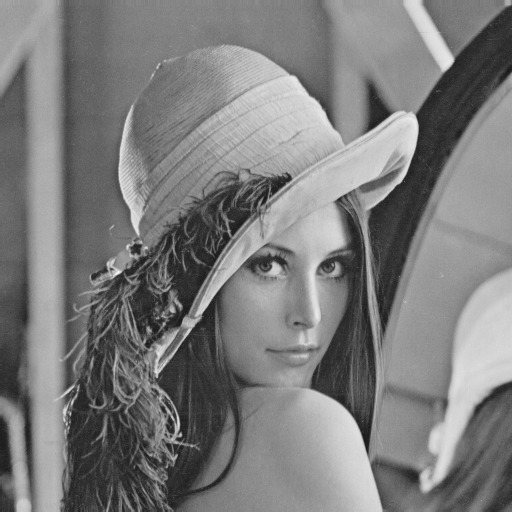
\includegraphics[width=0.5\columnwidth]{gray.jpg} % Example image
	\caption{Αρχική εικόνα.}
\end{figure}


Το εργαστήριο έχει ως σκοπό την εξοικείωση μας με την συνέλιξη σε δισδιάστατα σήματα όπως μια grayscale εικόνα συνελιγμένη με ένα δισδιάστατο kernel/φίλτρο.
Βλέπουμε τους λόγους που χρειάζεται να μεγαλώσουμε τις διαστάσεις μιας εικόνας ανάλογα το μέγεθος του φίλτρου και μελετάμε δύο διαφορετικές πρακτικές
padding. Συγκεκριμένα την συμπλήρωση με μηδενικά και την αντιγραφή των ακριανών pixel. Συγκρίνουμε τις πρακτικές αυτές μέσω της σηματοθορυβικής
σχέσης μεταξύ της αρχικής και παραγώμενης εικόνας, και του μέσου τετραγωνικού σφάλματος αντίστοιχα, όπως είδαμε και στο προηγούμενο εργαστήριο.
Επιπλέον, υλοποίηση γίνεται με την χρήση τριών διαφορετικούς συναρτήσεων.
\begin{enumerate}
  \item convolution(), η δική μας υλοποίηση της συνέλιξης δύο διαστάσεων.
  \item conv2(), η συνάρτηση του matlab για σήματα δύο διαστάσεων.
  \item imfilter(), η συνάρτηση του matlab για φιλτράρισμα εικώνων.
\end{enumerate}
Θεωρητικά, θα πρέπει και οι τρεις συναρτήσεις να παράξουν τα ίδια σφάλματα.
%------------------------------------------------

\subsection{Υλοποίηση της convolution}

Αρχικά από τις διαστάσεις της εικόνας με τα paddings και τις διαστάσεις του φίλτρου, υπολογίζουμε τις διαστάσεις της
καινούριας εικόνας. Έπειτα περιστρέφουμε το array του φίλτρου κατά 180$^{\circ}$ έτσι ώστε να γίνει η αναστροφή ``χιαστή''
που συζητήθηκε στο εργαστήριο. Τέλος, γεμίζουμε με μηδενικά τον πίνακα επιστροφής και ξεκινάμε τον υπολογισμό με δύο
εμφωλευμένα for loops. Για κάθε κελί του τελικού πίνακα, παίρνουμε ένα \textit{3x3} subsection του padded πίνακα και το
πολλαπλασιάζουμε στοιχείο-στοιχείο με το αναστραμένο φίλτρο.

\matlabscript {convolution}{Η υλοποίησή μας για την συνέλιξη}

\subsection{Υλοποίηση της padding}

Για την δημιουργία του πίνακα με τα επιπλέον περιθώρια, υλοποιήσαμε μια συνάρτηση η οποία δημιουργεί τέτοιες εικόνες για
οποιοδήποτε τετραγωνικό φίλτρο. Σε αυτήν, αρχικά υπολογίζουμε σύμφωνα με τους τύπους το καινούριο μέγεθος του πίνακα και
τον γεμίζουμε με μηδενικά. Έπειτα ελέγχουμε το κείμενο εισόδου, αν είναι \textit{zero}, τότε γεμίζουμε τα περιθώρια με μηδενικά
με την χρήση for loop, αν είναι \textit{fill}, κάνουμε replicate τα ακριανά pixel με χρήση της συνάρτησης padarray του
matlab, αλλιώς επιστρέφουμε σφάλμα.

\matlabscript {padForConv}{Η υλοποίησή μας για τα paddings}

\section{Συγκρίσεις και πειραματικά αποτελέσματα}

Αρχικά από την εικόνα μας, δημιουργούμε τα δύο διαφορετικά paddings με την χρήση της συνάρτησής μας. Έπειτα ακολουθεί
μια trivial διαδικασία, όπου παίρνουμε για κάθε μέθοδο padding και για κάθε συνάρτηση τις καινούριες εικόνες. Σε αυτό
το στάδιο παρατηρούμε ότι το γκαουσσιανό φίλτρο εξομαλύνει τα edges. Τελικά, με reference την αρχική μας εικόνα, και
με την χρήση των \textit{immse} και \textit{psnr}, εξάγουμε τις τιμες των σφαλμάτων.


Ας δούμε οπτικά τα αποτελέσματα.

\begin{figure}[h] % [h] forces the figure to be output where it is defined in the code (it suppresses floating)
	\centering
	\includegraphics[width=\columnwidth]{1.jpg} % Example image
	\caption{Με την χρήση της μεθόδου μας.}
\end{figure}

\begin{figure}[h] % [h] forces the figure to be output where it is defined in the code (it suppresses floating)
	\centering
	\includegraphics[width=\columnwidth]{2.jpg} % Example image
	\caption{Με την χρήση της conv2().}
\end{figure}

\begin{figure}[h] % [h] forces the figure to be output where it is defined in the code (it suppresses floating)
	\centering
	\includegraphics[width=\columnwidth]{3.jpg} % Example image
	\caption{Με την χρήση της imfilter().}
\end{figure}


\clearpage
\newpage

\section{Τελικά αποτελέσματα}

Επιβεβαιώνεται η θεωρητική μας πρόβλεψη. Όλες οι συναρτήσεις δημιουργούν τις ίδιες εικόνες και άρα
τα σφάλματα είναι κοινά για κάθε μέθοδο.
\begin{table}[h] % [h] forces the table to be output where it is defined in the code (it suppresses floating)
	\centering % Centre the table
	\begin{tabular}{l c c c}
		\toprule
		\textit{σφάλμα/padding} & \textbf{convolute()} & \textbf{conv2()} & \textbf{imfilter()} \\
		\midrule
		\midrule
		MSE (zero) & 25.25 & 25.25 & 25.25 \\
		MSE (fill) & 17.24 & 17.24 & 17.24 \\
		\midrule
		PSNR (zero) & 34.11 & 34.11 & 34.11 \\
		PSNR (fill) & 35.76 & 35.76 & 35.76 \\
		\bottomrule
	\end{tabular}
	\caption{Τα τελικά σφάλματα.}
\end{table}

\begin{figure}[h] % [h] forces the figure to be output where it is defined in the code (it suppresses floating)
	\centering
	\includegraphics[width=\columnwidth]{4.jpg} % Example image
	\caption{Ενδεικτικά, το output της εεφαρμογής μας στην κονσόλα του matlab.}
\end{figure}


\section{Σύγκριση των τριών συναρτήσεων.}

Εφ' όσων στην δική μας υλοποίηση κάνουμε περιστροφή του φίλτρου και βγάζουμε ίδια σφάλματα μπορούμε
να συμπεράνουμε ότι η μεθοδολογία αυτή είναι κοινή και για τις άλλες δύο συναρτήσεις.


Για κοινές εξόδους από τις συναρτήσεις, ας συγκρίνουμε τις εισόδους
\begin{enumerate}
  \item \textbf{convolution()} Παίρνει ως είσοδο την εικόνα \underline{με} τα paddings και το φίλτρο.
  \item \textbf{conv2()} Παίρνει ως είσοδο την εικόνα \underline{με} τα paddings και το φίλτρο καθώς
  και ένα string ``valid'' με το οποίο ζητάμε να γίνει η συνέλιξη όπως την συζητήσαμε και να μην μας
  επιστρέψει εικόνα ίδιου μεγέθους με αυτή με τα paddings.
  \item \textbf{convolution()} Παίρνει ως είσοδο την εικόνα \underline{χωρίς} τα paddings και το φίλτρο.
  Επιστρέφει πάντα εικόνα ίδιου μεγέθους με την αρχική και μέσω ενός string ορίζει την μέθοδο για τα
  paddings (``replicate'') ή έναν αριθμό (0) για την τιμή των επιπλέων pixel. Τέλος χρειάζεται το string
  ``conv'' για να κάνει συνέλιξη και όχι καποια άλλη πράξη.
\end{enumerate}

\section{Ο κώδικας που υλοποίησε τα παραπάνω}

\matlabscript {main}{Η υλοποίηση σε Matlab}

\end{document}
